\begin{frame}{Gruppen (1)}
Warum Gruppen?

\pause
Gruppen
\begin{itemize}
\item beschreiben Symmetrien
\pause
\item sind nützlich
\pause
\item sind interessant
\end{itemize}
\end{frame}

\note{
Anwendungen
\begin{itemize}
\item Schwarze Löcher
\item Kryptographie (Verschlüsselung)
\item Versuchsdesign
\item $\ldots$
\end{itemize}
}

\begin{frame}{Gruppen (2)}
\begin{columns}
\begin{column}{0.4\textwidth}
\vspace{6.65em}
\end{column}
\begin{column}{0.5\textwidth}
\begin{center}
  \animategraphics[]{9}{animation/}{1}{9}
\end{center}
\end{column}
\end{columns}
\vspace{1.4em}
\end{frame}

\begin{frame}[noframenumbering]{Gruppen (2)}
\begin{columns}
\begin{column}{0.4\textwidth}
\pause
Vier Eigenschaften
\begin{itemize}
\pause
\item Neutrales Element
\pause
\item Abgeschlossen
\pause
\item Invertierbar
\pause
\item Assoziativ
\end{itemize}
\end{column}
\begin{column}{0.5\textwidth}
\begin{center}
  \animategraphics[]{12}{animation/}{1}{17}
\end{center}
\end{column}
\end{columns}
\vspace{-2em}
\pause
Gruppe die aus Vertauschungen besteht:
\emph{Permutationsgruppe}.

\pause
\emph{Disclaimer:} hier nur endliche Gruppen und Mengen!
\end{frame}

\note{
Eine Anwendung der Gruppentheorie:
Eigenschaften des Objekts davon ableiten, wie die Symmetrien miteinander
interagieren.
}

\begin{frame}{Klassifikation endlicher einfacher Gruppen}
%Was sind die kleinsten Bausteine\footnote{math.: einfache Gruppen} der Gruppen?
%
\pause
\begin{figure}[h]
\centering
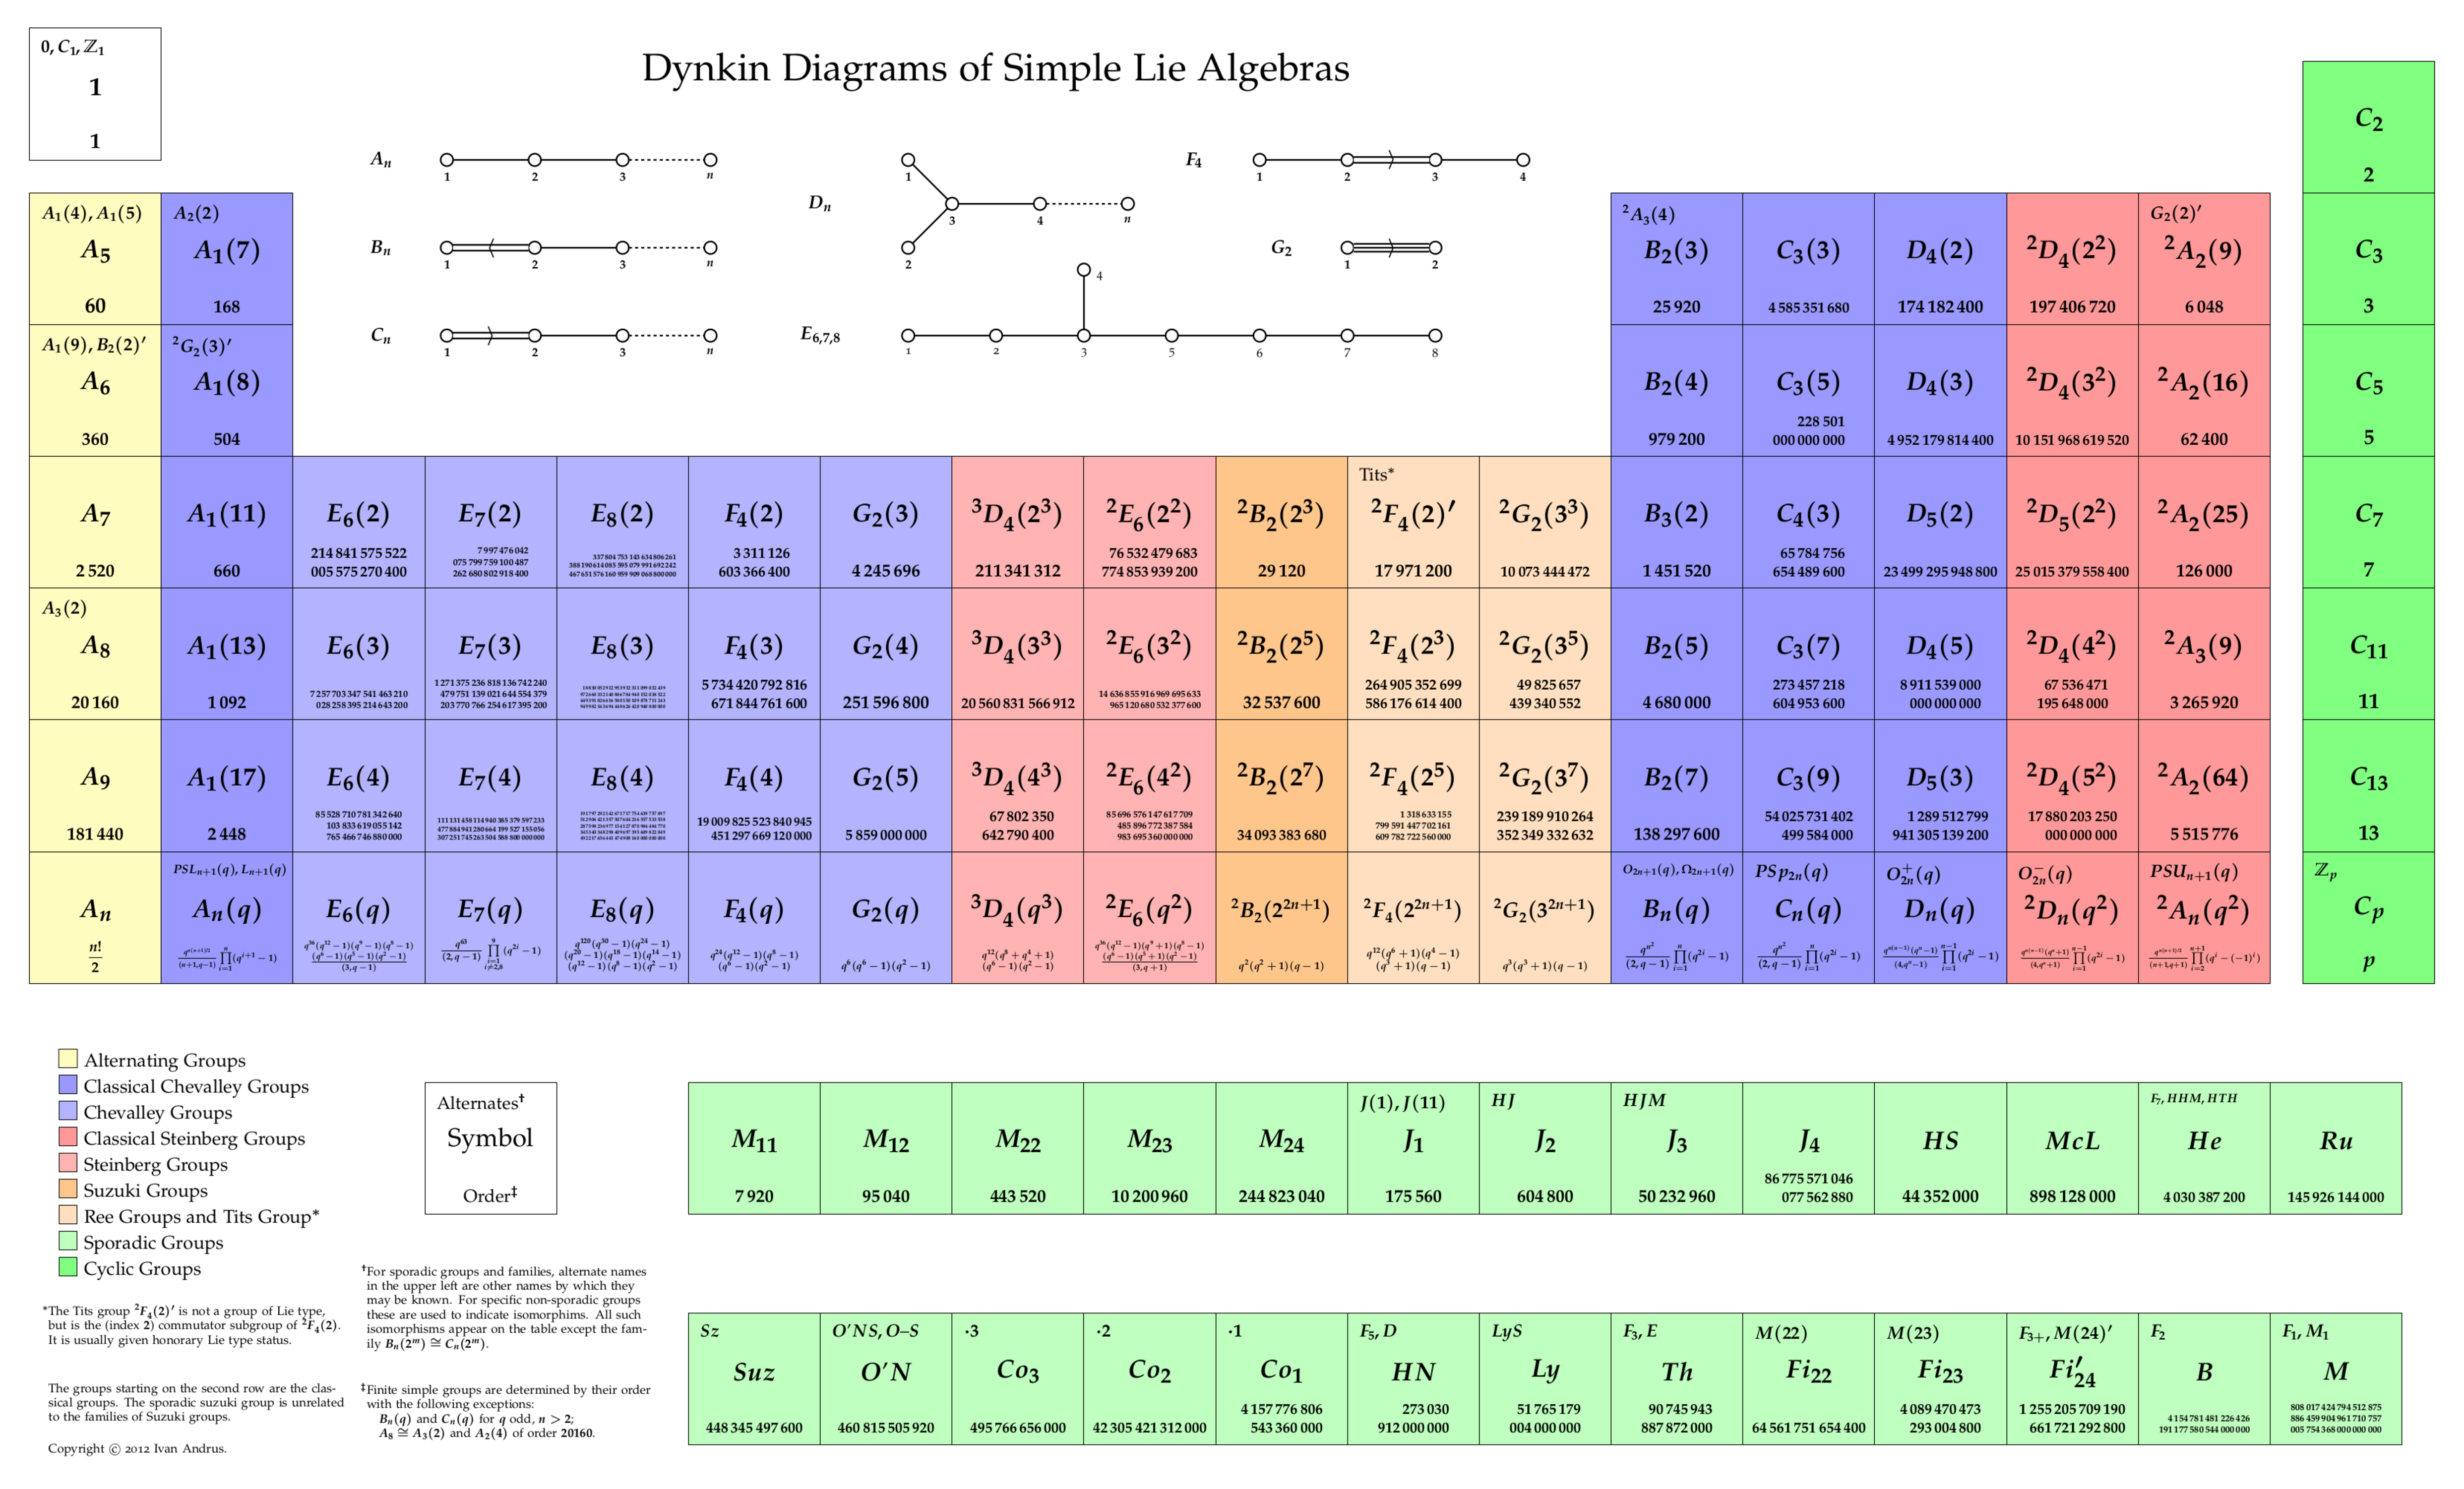
\includegraphics[width=0.9\textwidth]{./pictures/periodic-table-of-groups-cropped.pdf}
\caption{Periodensystem endlicher einfacher Gruppen%
\footnote{By Ivan Andrus, from
\href{https://irandrus.wordpress.com}{irandrus.wordpress.com}}
}
\end{figure}
\end{frame}

\note{
Klassifikation ist einer der Stützpfeiler
}

\begin{frame}{Normalisatoren}
Normalisatoren%
\footnote{$G, M \leq K$.
Normalisator von $G$ in $M$ ist
$N_M(G) = 
\set{ m \in M ~|~ G ^ m = G }
$.
}:

\begin{itemize}
\item Werkzeuge um Gruppen zu verstehen
\pause
\item für beliebige Gruppen schwer zu berechnen
\pause
\item kein effizienter Algorithmus bekannt
\end{itemize}
\end{frame}

%\begin{frame}{Experimente}
%Untersuchung mithilfe von Computern
%\begin{itemize}
%\item Manche Fragen können einfach beantwortet werden $\ldots$
%\item $\ldots$ andere hingegen nur mit großem Aufwand.
%\end{itemize}
%\end{frame}

\begin{frame}{Wie schwer?}
Bester bekannter allgemeiner Algorithmus:
einfach exponentielle Laufzeit $2 ^ {O(n)}$ von Daniel Wiebking.

\pause
\begin{figure}[h]
\centering
\includegraphics[width=0.3\textwidth]{./pictures/The_Sun.jpg}
\caption{Sonne%
\footnote{The Sun, By NASA/SDO (AIA) - Public Domain}
}{Sonn}
\end{figure}
\end{frame}

\note{Überleitung:
Was macht man, wenn man ein großes Problem nicht lösen kann? Man sucht
sich ein einfacheres.
}

\begin{frame}{Primitive Gruppen}
\pause
Eine transitive Permutationsgruppe $G \leq \sym \Omega$ heißt
\emph{imprimitiv},
\pause
falls es eine nicht-triviale
$G$-invariante Partition von $\Omega$ gibt,
\pause
sonst \emph{primitiv}.

\pause
\begin{figure}[h]
\centering
\includegraphics[width=0.3\textwidth]{./pictures/787px-Freerange_eggs_cropped.jpg}
~
\includegraphics[width=0.3\textwidth]{./pictures/787px-Freerange_eggs_cropped.jpg}
\caption{Partition von Eiern%
\footnote{``Freerange eggs.jpg'' cropped - Wikimedia Commons - CC BY-SA 3.0}
}
\end{figure}
\end{frame}

\note{
Wie lässt sich eine Permutationsgruppe zerlegen?

Kleinsten Bausteine der Permutationsgruppen sind primitive.
}

\section{Resultat}
\begin{frame}%{Resultat}
\begin{block}{Satz}
Sei \textcolor{blue}{$G = \gen X \leq \sym \Omega$ eine primitive Gruppe
mit nicht-regulärem Sockel}.
\pause
Dann kann ein
\textcolor{orange}{Erzeugendensystem von $N_{\sym \Omega}(G)$}
\pause
in
\textcolor{green}{Zeit polynomiell beschränkt in $\abs X$ und $\abs
\Omega$} bestimmt werden.
\end{block}
\vspace{1.5em}
\pause
Beachte: Für $M \leq \sym \Omega$ gilt
$N_{M}(G) = M \cap N_{\sym \Omega}(G)$.
\end{frame}

\note{
Erwähnen?:
Hoffnung:
bessere Algorithmen für "zusammengesetzte" Gruppen.
}

\section{Strategie}
\note{Struktur primitiver Gruppen ausnutzen}
\begin{frame}{Permutationsisomorphie}
Notation: $\omega ^ g := g(\omega)$.
\vspace{2em}

Zwei Gruppen $G \leq \sym \Omega$ und $H \leq \sym \Delta$ heißen
\emph{permutationsisomorph}, wenn
Isomorphismen $f : \Omega \to \Delta$ und $\phi : G \to H$ existieren,
sodass
$\forall g \in G, \omega \in \Omega$:
\[
    f( \omega ^ g ) = f(\omega) ^ {\phi(g)}.
\]
\end{frame}

\begin{frame}{Struktursatz primitiver Gruppen}
Der \emph{Sockel} einer Gruppe $G$, geschrieben
$\soc G$, ist das Erzeugnis aller minimalen Normalteiler von $G$.

\pause
Der Sockel einer primitiven Gruppe ist charakteristisch einfach.

\pause
\begin{block}{Satz von O'Nan-Scott}
Sei $G \leq \sym \Omega$ eine primitive Permutationsgruppe.
Bis auf Permutationsisomorphie kennen wir
\begin{itemize}
\item $\soc G$,
\item $N_{\sym \Omega}( \soc G )$.
\end{itemize}
\end{block}
\end{frame}

\begin{frame}{Hauptschritte}
Sei $G \leq \sym \Omega$ eine primitive Permutationsgruppe.
Berechne $N_{\sym \Omega}(G)$.

\pause
Bestimme
\begin{itemize}
\item $M := N_{\sym \Omega}(\soc G)$.
Es gilt $N_{\sym \Omega}(G) = N_M(G)$.

\pause
\item Gruppenhom.
$
    \rho : M \to S_k
$
mit $k \in O(\log \abs \Omega)$.
%und
%\[
%    N_{\sym \Omega}(G) = N_{M}(G) = \rho ^ {-1}( N_{\rho(M)}(\rho(G)) ).
%\]
\end{itemize}
\end{frame}

\note{
Log. Reduktion einfach. Dann im Endeffekt nur Algorithmus von Daniel Wiebking.

Normalisator des Sockels mehr Aufwand.
}

%\begin{frame}{Logarithmische Reduktion}
%Kranzprodukt in Produktoperation
%$\rightarrow$
%imprimitive Operation
%
%\pause
%Sockel herausfaktorisieren
%\end{frame}
%
%\note{
%Produkt $\rightarrow$ imprimitiv macht $d ^ \ell$ zu $d \cdot \ell$ Punkten.
%
%Kranzprodukt:
%\begin{itemize}
%\item Symmetrische Gruppe auf Anzahl Komponenten von $\Omega ^ {\ast}$.
%\item Sockel einfache Gruppen + äußere Automorphismen.
%Nach herausfaktorisieren des Sockels bleiben nur die äußeren Automorphismen.
%\end{itemize}
%
%Wichtig:
%$\log ^ 2(n)$ würde nur quasipolynomiellen Algorithmus liefern.
%}
